% Author:Zhuming Shi, Peking University
% Theme from https://github.com/matze/mtheme

% \documentclass[12pt,AutoFakeBold,aspectratio=169,mathserif]{beamer}
\documentclass[12pt,AutoFakeBold,aspectratio=43,mathserif]{beamer}
\usepackage[english]{babel}

\usetheme{metropolis}

\usepackage{fontspec}% 控制字体
\setmainfont{Times New Roman}% 英文字体
\newfontfamily\arial{Arial}% Arial字体

\usepackage{xeCJK} % 中文支持
\setCJKmainfont{SimSun} % 中文字体
\XeTeXlinebreaklocale "zh"%中文自动换行
\XeTeXlinebreakskip = 0pt plus 1pt%中文自动换行

\usepackage{graphicx}
\usepackage{subfigure}
\usepackage{caption}

\usepackage{amsthm,amsmath,amssymb,mathrsfs}% 数学符号和花体支持
\usepackage{booktabs}% 绘制三线表
\usepackage{latexsym}% 绘制特殊数学符号
\usepackage{siunitx}% 数学模式中使用SI单位

\usepackage[version=3]{mhchem}% 化学反应式
\usepackage{epstopdf}% 插入ChemDraw的.eps结构图

% 代码环境
\usepackage{listings}
\usepackage{color}

\definecolor{dkgreen}{rgb}{0,0.6,0}
\definecolor{gray}{rgb}{0.5,0.5,0.5}
\definecolor{mauve}{rgb}{0.58,0,0.82}

\lstset{frame=tb,
  language=c++,
  aboveskip=3mm,
  belowskip=3mm,
  showstringspaces=false,
  columns=flexible,
  basicstyle={\small\ttfamily},
  numbers=none,
  numberstyle=\tiny\color{gray},
  keywordstyle=\color{blue},
  commentstyle=\color{dkgreen},
  stringstyle=\color{mauve},
  breaklines=true,
  breakatwhitespace=true,
  tabsize=3
}

\setbeamerfont{footnote}{size=\tiny}

\newcommand{\unknow}[1]{{\arial \textbf{#1}}}%未知化合物格式
\newcommand{\substance}[1]{\textbf{\emph{#1}}}%矿物名称格式

% \setbeamertemplate{background}{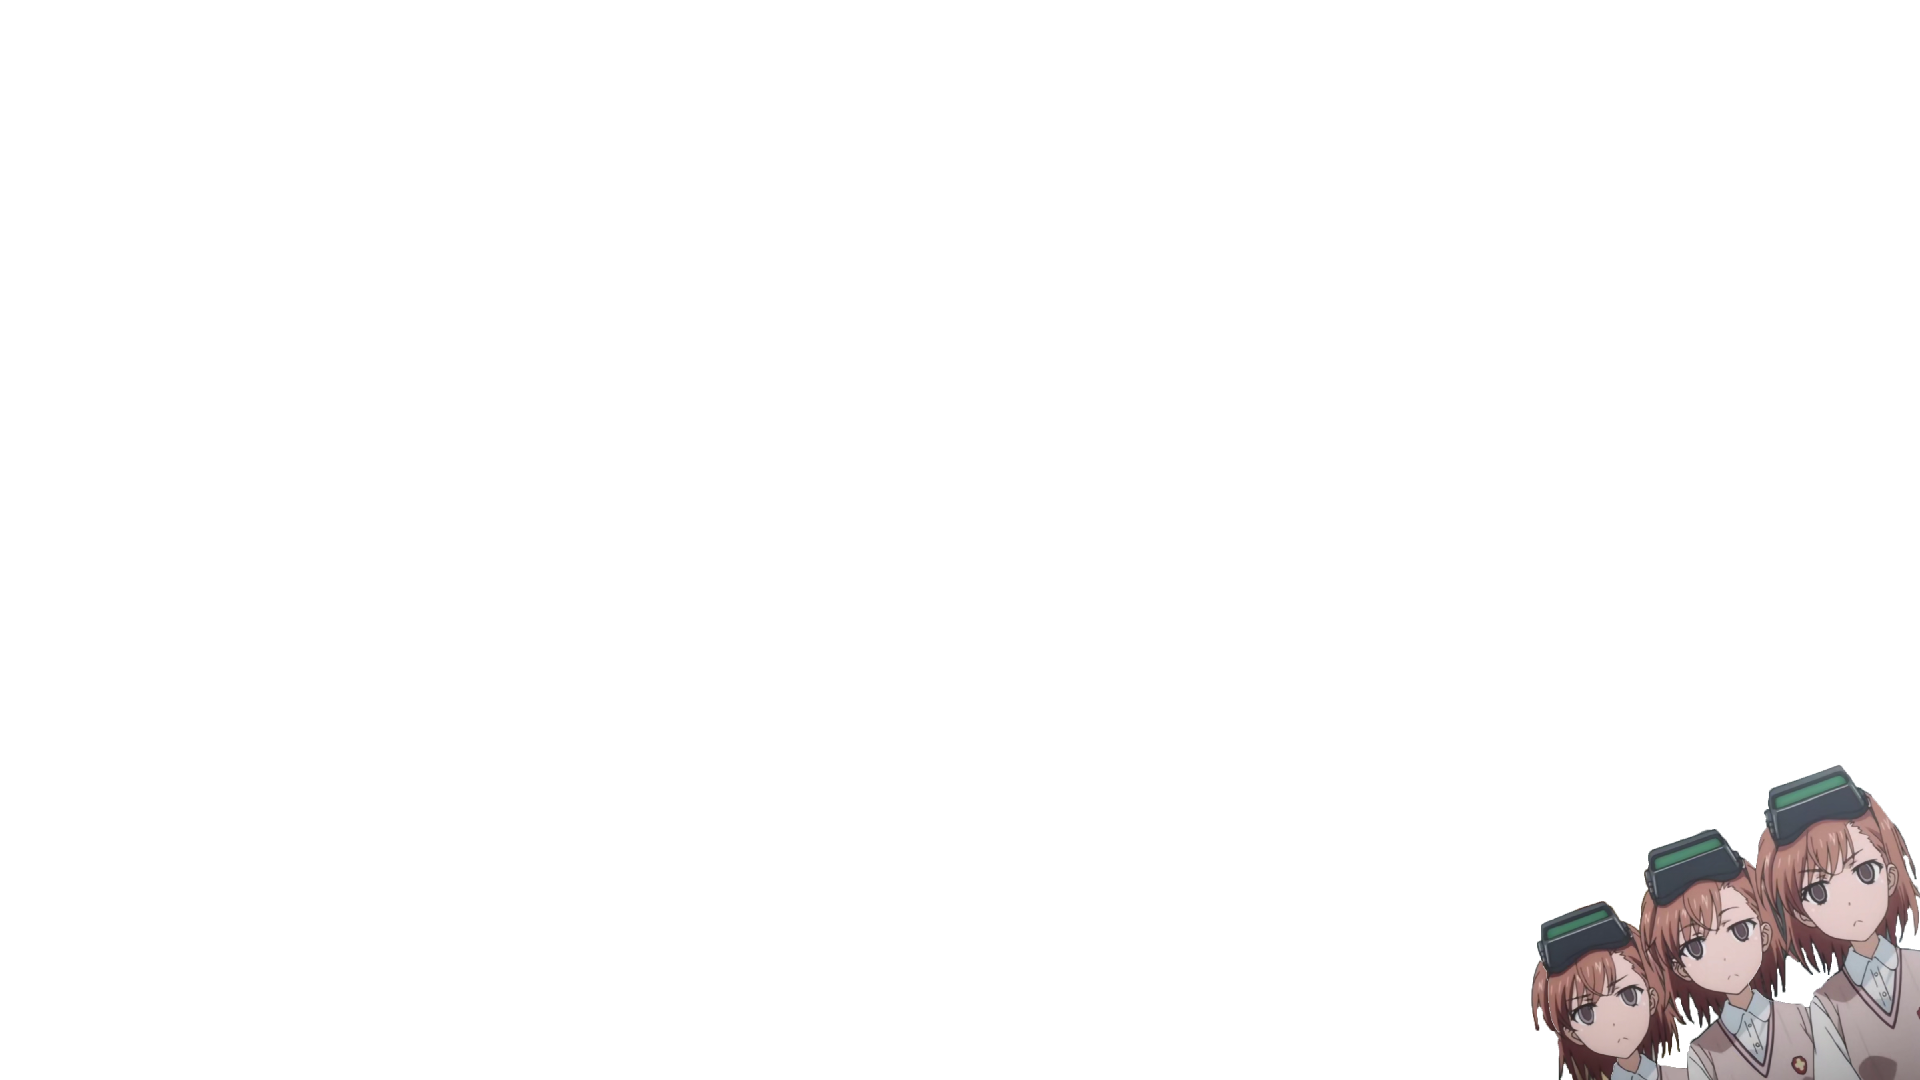
\includegraphics[height=\paperheight]{figures/sisters1080.png}}

\makeatletter 
\renewcommand{\@thesubfigure}{\hskip\subfiglabelskip}
\makeatother

\title{网络编程3}
\author{施朱鸣}
\date{12月24日}

\begin{document}
    {
    % \setbeamertemplate{background}{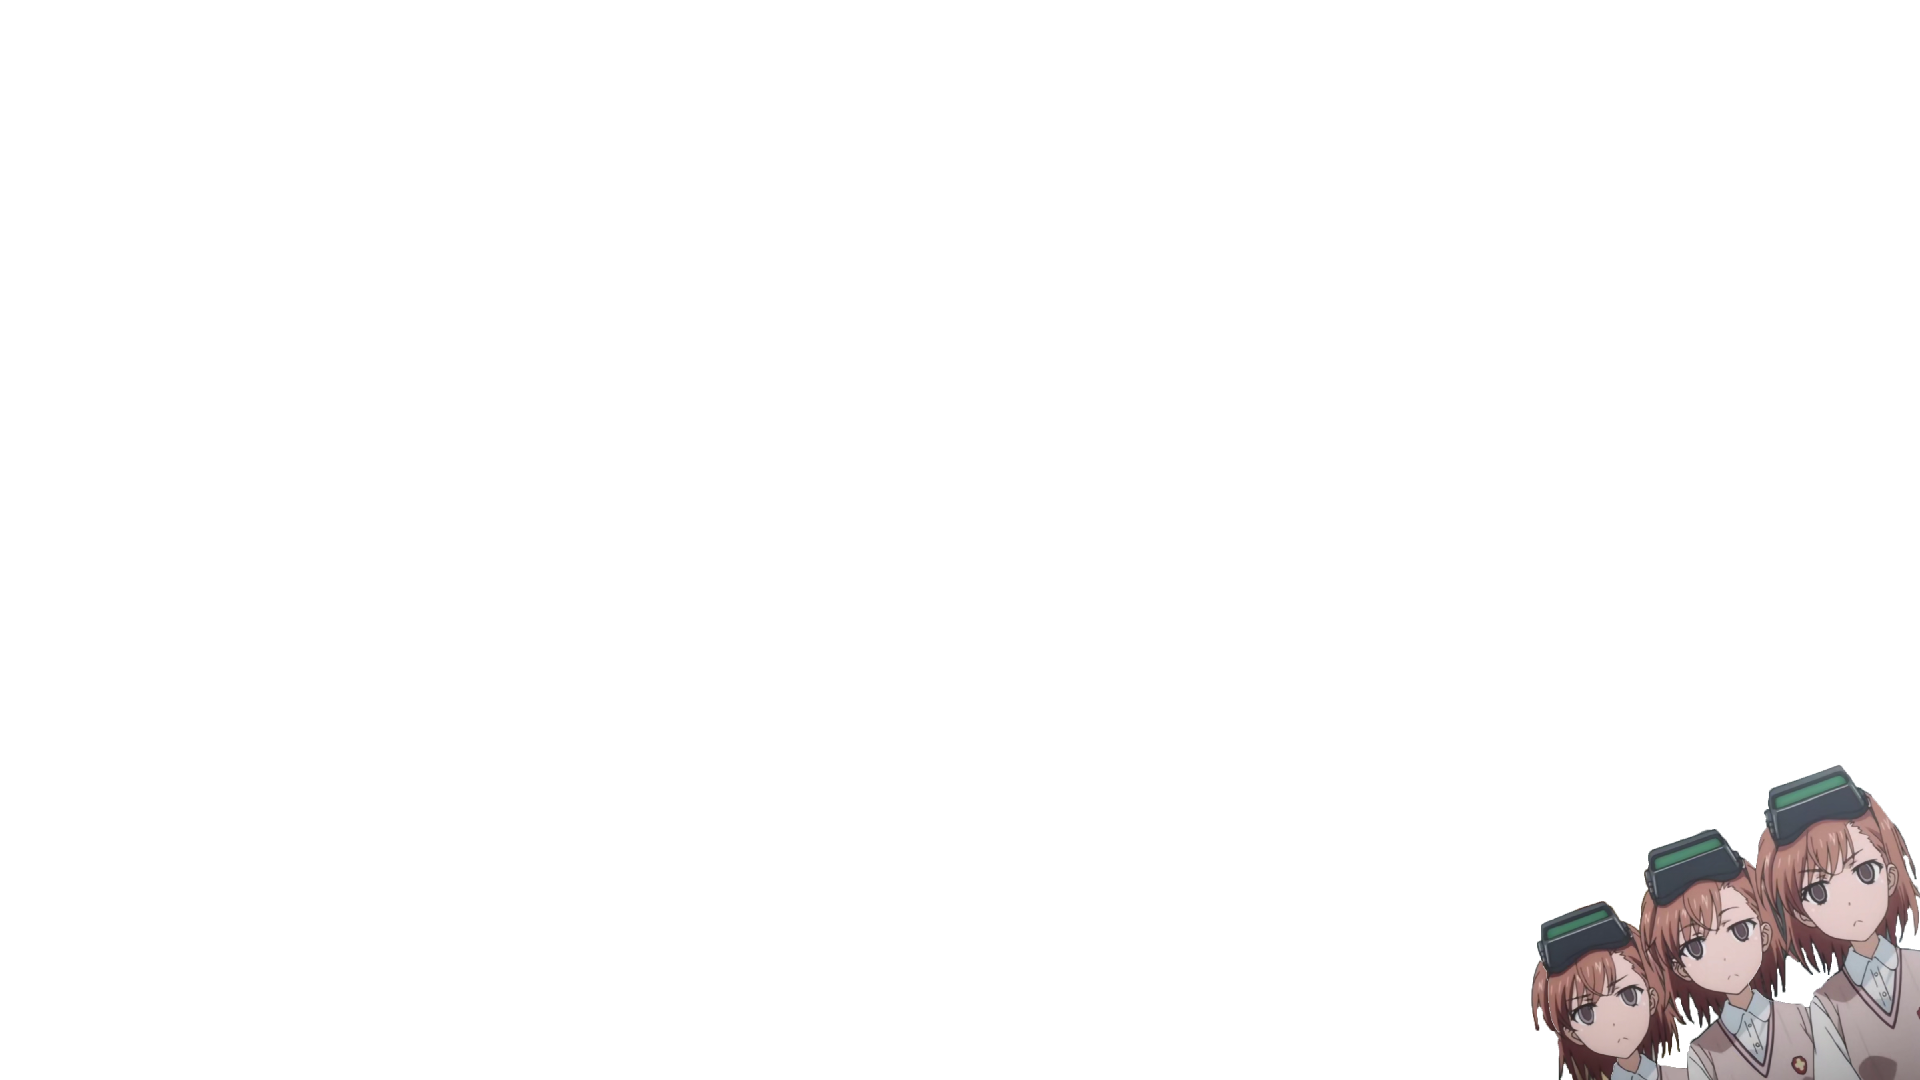
\includegraphics[height=\paperheight]{figures/sisters1080.png}}
    % \setbeamertemplate{background}{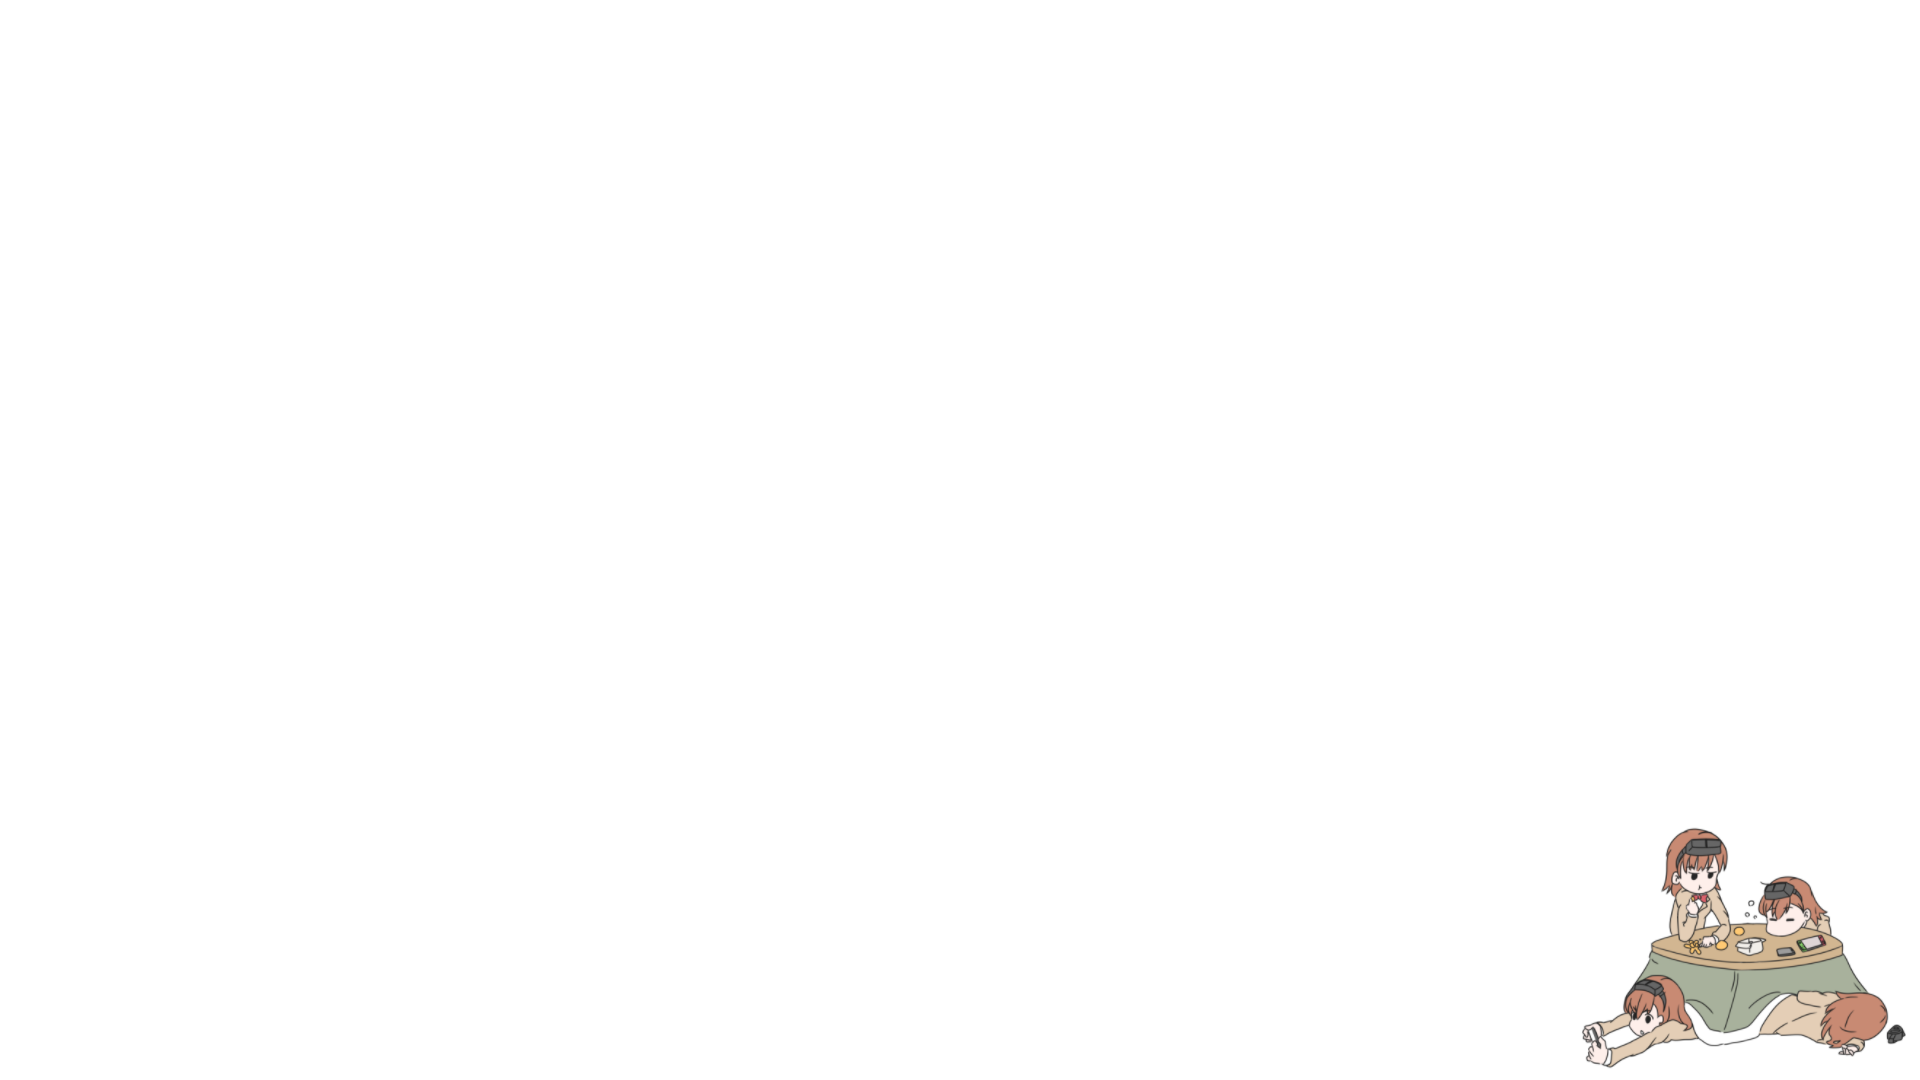
\includegraphics[height=\paperheight]{figures/misaka1080.jpg}}
    \setbeamertemplate{background}{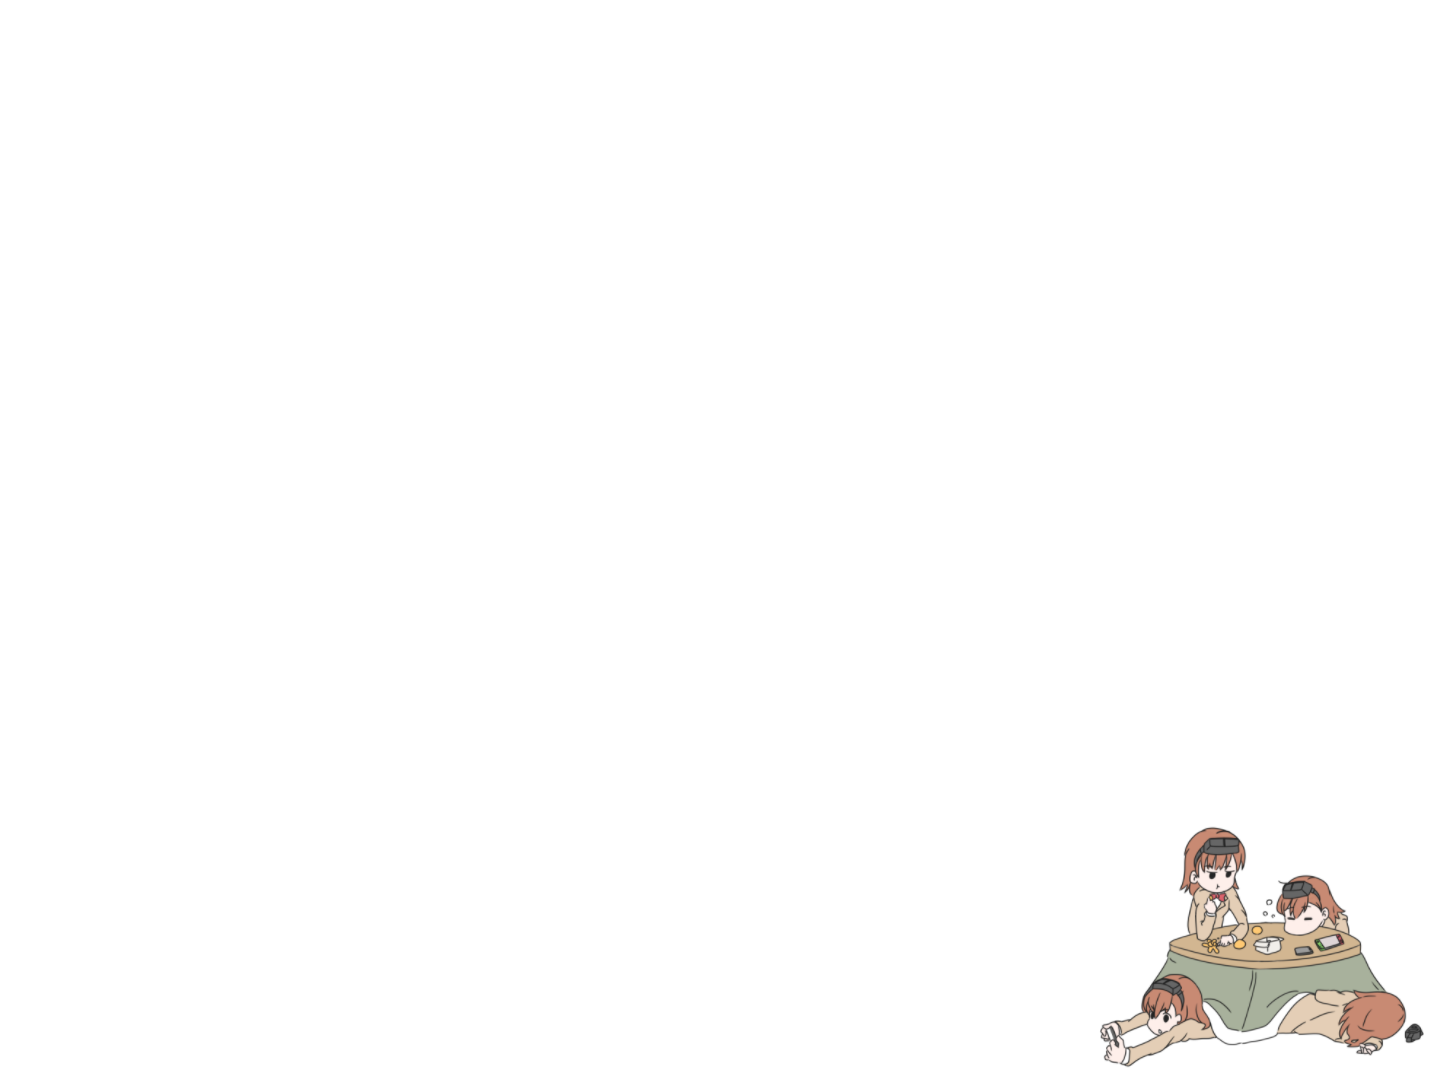
\includegraphics[height=\paperheight]{figures/misaka43.jpg}}
    
    \begin{frame}
    \titlepage
    \end{frame}
    \frame{\frametitle{Outline}\tableofcontents[hideallsubsections]}

    \section{网络请求}
    \begin{frame}
        \frametitle{怎么进行HTTP传输?}
    
        \begin{itemize}
            \item 超文本传输协议\begin{itemize}
                \item 超在哪里?可以包含超链接<a herf="..."> </a>
            \end{itemize}
            \item 四步走\begin{itemize}
                \item 建立TCP连接
                \item 客户端请求内容
                \item 服务器回复
                \item 关闭连接
            \end{itemize}
        \end{itemize}

    \end{frame}

    \begin{frame}
        \frametitle{传输什么样的内容?}
    
        \begin{itemize}
            \item 静态内容\begin{itemize}
                \item html页面等已有的内容->直接发过去
                \item 类比printf("Hello world!");
            \end{itemize}
            \item 动态内容\begin{itemize}
                \item 需要运行程序才能知道发送什么->fork一下并运行
                \item 类比printf("\%ld",time());
            \end{itemize}
            \item web内容与服务器上的文件相联系
        \end{itemize}
    
    \end{frame}

    \begin{frame}
        \frametitle{动态内容怎样传递参数?}
    
        \begin{itemize}
            \item 一切web内容利用URL来定位(类比指针)
            \item 静态内容:\begin{itemize}
                \item 写明http://pkuszm.cn/index.html则发送这个文件
                \item 只写http://pkuszm.cn/则发送默认文件
            \end{itemize}
            \item 动态内容:https://cn.bing.com/search?q=清华大学\begin{itemize}
                \item 通常长成...?...=...这个样子
            \end{itemize}
        \end{itemize}
    
    \end{frame}

    \begin{frame}
        \frametitle{http请求}
    
        \begin{itemize}
            \item 一个请求行+任意个请求报头
            \item 请求行<method> <uri> <version>\begin{itemize}
                \item <method> GET, POST, OPTIONS, HEAD, PUT, DELETE, TRACE
                \item <uri> 广义的url,类比地址
                \item <version> HTTP/1.0或者HTTP/1.1
            \end{itemize}
            \item 请求报头<header name>: <header data>\begin{itemize}
                \item 额外的信息,例如浏览器叫chrome
            \end{itemize}
        \end{itemize}
    
    \end{frame}
    
    \section{小型服务器的实现}

    \section{代理}
    
    \section*{致谢}}

    \begin{frame}
        \setbeamertemplate{background}{}
        \frametitle{致谢}
        \begin{columns}
            \begin{column}{.5\linewidth}
                祝大家圣诞快乐!谢谢聆听!
            \end{column}
            \begin{column}{.5\linewidth}
                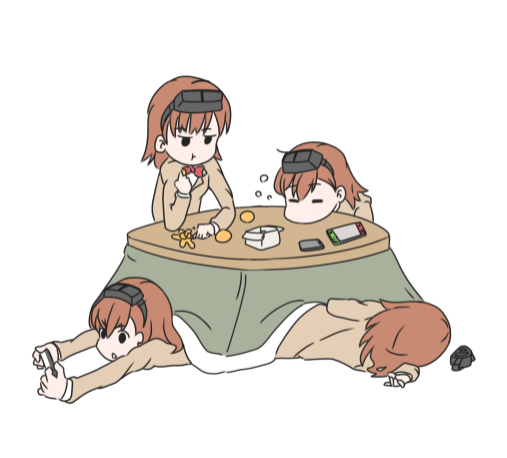
\includegraphics[width=.4\paperwidth]{figures/misaka558.png}
            \end{column}
        \end{columns}
    \end{frame}
    
\end{document}